In this part of the thesis, we report the results from the experiments. Since there are no direct benchmarks, it is vital to know how to view the results. In the simplest form, successful results can be stated when betting is profitable. Unfortunately, this is a very narrow perspective, and for that reason, we will dig deeper to understand why some of the models generate profitable returns. Also, it is important to know what downsides these models and strategies might have.  In short, Results section will answer to these questions 1) "Is it possible to bet on a FIFA World tournament profitably?",  2) "What are the main differences between the models?", 3) "How using different feature sets affect the results?", and 4) "How are the individual matches betted and how betting differs between tournaments?" During early experiments \textit{OVR model} with Platt scaling outperformed the vanilla model and the isotonic scaling. In the results \textit{OVR model} uses only Platt scaling.

\section{Tournament simulation results}
Tournament simulation results for each of the models are listed in Tables \ref{table:outcomemodel}, \ref{table:scoreresults}, \ref{table:onevsrestresults} and \ref{table:linearmodel}. The tables include metrics for accuracy, log loss, unit strategy's profit and Kelly strategy's profit. Listed values are averages from 10 individual simulations and include standard deviations. All metrics are listed for every feature set used in training. Abbreviations are used for feature set names: AF means \textit{all features}, GF means \textit{general features} and PF means \textit{player features}. Description for each of the feature set is listed in Table \ref{table:featuresetlist}.

To answer the question "Is it possible to bet on a FIFA World tournament profitably?" it is important to see if any of the models can generate profit. Preferably, a model should be profitable in each of the tournaments, since investors prefer steady profits. Also, if the model, trained using different data periods, can continuously keep its performance it is harder to say that the model was just lucky all the time.

Unit strategy's profits for \textit{Outcome mode}, \textit{Score model} and \textit{OVR model} are positive in every tournament, but not with all of the feature sets. Good profits from the unit strategy and high accuracy go hand in hand, which is no surprise. However, high accuracy is not an indicator for good Kelly profits, which is a slight of a surprise. When estimated probabilities are closer to the true ones than the market's probabilities, Kelly criterion is a working strategy. Since Kelly criterion aims to maximize the logarithm of expected wealth, it utilizes current bank more efficiently. The unit strategy uses just a static bet size of one unit per game and is not able to maximize all of the good opportunities. From the tested models only \textit{Outcome model}, trained with player features, is profitable with both of the strategies.

Bookmaker's accuracy on the World cup 2018 and the World cup 2014 was 56.25\% (36 games correctly predicted) and 51.56  \% (33 games correctly predicted) on the World cup 2010. Most of the models can outperform the bookmaker's model's accuracy, which is a promising result.

But which of the feature set and model combinations is the best? This question is tricky to answer. If being profitable in every tournament with a high profit is preferred then \textit{Score model}, trained with all features, might be the right choice. Whereas highest unit strategy's profit is achieved with \textit{OVR model} trained with player features. Using only these metrics to validate if a model is good enough to be trusted in the next World cup 2022 is too risky. Being profitable in 192 games (64 games per a tournament) is a good start.

\begin{table}
    \caption{Tournament characteristics. \textit{Underdog victory} is a case where the winning team has higher odds for winning than the other team. All of the tournaments have 64 games in total.}
    \begin{tabular}{| c | c|c | c|}
        \hline
        Characteristic & \textbf{WC 2018} & \textbf{WC 2014} & \textbf{WC 2010}\\
        \hline
        Home wins & 25 & 28 & 24\\
        Draws & 14 & 13 & 16\\
        Away wins & 25 & 23 & 24\\
        Underdog victory  & 14 & 15 & 14\\
        \hline
    \end{tabular}
    \label{table:tournamentcharacteristics}
\end{table}


\begin{table}
    \caption{Simualtion results for \textit{Outcome model}.}
    \resizebox{\linewidth}{!}{
        \begin{tabular}{| c  c| c| c| c|c|}
            \hline
            Metric& & \textbf{WC 2018} & \textbf{WC 2014} & \textbf{WC 2010} & Mean\\
            \hline
            Accuracy & AF & 57.34\% $\pm$ 0.72 & \textbf{60.94\% $\pm$ 1.71} & 54.84\% $\pm$ 1.09& 57.71 \\
             & GF & 52.03\% $\pm$ 1.22 & 56.56\% $\pm$ 0.62 & \textbf{55.47\% $\pm$ 1.05} & 54.69 \\
             & PF & \textbf{60.47\% $\pm$ 1.41} & 59.69\% $\pm$ 0.94 & 54.22\% $\pm$ 2.22& \textbf{58.13} \\
             & & & & & \\
            Log Loss & AF & 0.9673 $\pm$ 0.0037 & \textbf{0.9362 $\pm$ 0.0047} & 0.9922 $\pm$ 0.0075& \textbf{0.9652} \\
             & GF & 1.0122 $\pm$ 0.0045 & 0.9549 $\pm$ 0.0053 & \textbf{0.9676 $\pm$ 0.0052}& 0.9782 \\
             & PF & \textbf{0.9406 $\pm$ 0.0026} & 0.9503 $\pm$ 0.0024 & 1.0118 $\pm$ 0.0045& 0.9676 \\
             & & & & & \\
            Unit profit & AF & 6.39\% $\pm$ 1.96 & \textbf{15.65\% $\pm$ 5.21} & 2.93\% $\pm$ 4.43& 8.32 \\
             & GF & -3.48\% $\pm$ 3.4 & 5.17\% $\pm$ 1.52 & \textbf{5.04\% $\pm$ 3.67}& 2.24 \\
             & PF & \textbf{18.38\% $\pm$ 4.26} & 12.72\% $\pm$ 2.22 & 3.32\% $\pm$ 8.33&\textbf{ 11.47 }\\
             & & & & & \\
            Kelly profit & AF & -10.58\% $\pm$ 7.01 & \textbf{18.55\% $\pm$ 10.13} & 23.26\% $\pm$ 18.96& 10.41 \\
             & GF & -47.32\% $\pm$ 4.1 & 2.86\% $\pm$ 8.15 & \textbf{48.9\% $\pm$ 16.64}& 1.48 \\
             & PF & \textbf{46.63\% $\pm$ 8.79} & 12.26\% $\pm$ 6.57 & 2.75\% $\pm$ 9.05& \textbf{20.55 }\\
        \hline
        \end{tabular}
    }
    \label{table:outcomemodel}
\end{table}


\begin{table}
    \caption{Simulation results for \textit{Score model}.}
    \resizebox{\linewidth}{!}{
    \begin{tabular}{| c  c| c| c| c|c|}
        \hline
        Metric& & \textbf{WC 2018} & \textbf{WC 2014} & \textbf{WC 2010} & Mean\\
        \hline
        Accuracy & AF & \textbf{59.38\% $\pm$ 0.0} & 58.13\% $\pm$ 0.62 & 52.81\% $\pm$ 0.62& 56.77 \\
         & GF & 52.03\% $\pm$ 1.0 & \textbf{59.38\% $\pm$ 0.0} & 50.94\% $\pm$ 0.77& 54.12 \\
         & PF & 58.44\% $\pm$ 1.74 & 61.09\% $\pm$ 0.84 & \textbf{53.91\% $\pm$ 0.78}& \textbf{57.81} \\
         & & & & & \\
        Log Loss & AF & \textbf{0.9508 $\pm$ 0.0016} & 0.935 $\pm$ 0.0005 & 0.9788 $\pm$ 0.0016& 0.9549 \\
         & GF & 0.9831 $\pm$ 0.0012 & \textbf{0.9133 $\pm$ 0.0011} & \textbf{0.9522 $\pm$ 0.001} & \textbf{0.9495} \\
         & PF & 0.9566 $\pm$ 0.0013 & 0.9446 $\pm$ 0.0024 & 0.9996 $\pm$ 0.0009& 0.9669 \\
         & & & & & \\
        Unit profit & AF & \textbf{13.52\% $\pm$ 0.0} & 5.94\% $\pm$ 2.11 & -2.8\% $\pm$ 1.29& 5.55 \\
         & GF & -5.4\% $\pm$ 2.57 & 13.66\% $\pm$ 0.0 & -5.08\% $\pm$ 2.45& 1.06 \\
         & PF & 12.26\% $\pm$ 5.1 & \textbf{16.11\% $\pm$ 2.64} & \textbf{2.23\% $\pm$ 2.09} & \textbf{10.2 }\\
         & & & & & \\
        Kelly profit & AF & \textbf{35.59\% $\pm$ 4.45} & 12.37\% $\pm$ 1.02 & 24.2\% $\pm$ 4.43& 24.05 \\
         & GF & -19.06\% $\pm$ 1.87 & \textbf{107.61\% $\pm$ 4.47} & \textbf{99.75\% $\pm$ 3.63} & \textbf{62.77} \\
         & PF & 2.04\% $\pm$ 2.62 & 10.82\% $\pm$ 4.87 & 8.3\% $\pm$ 2.1& 7.05 \\
 \hline
    \end{tabular}}
    \label{table:scoreresults}
\end{table}

\begin{table}
    \caption{Simulation results for \textit{OVR model}.}
    \resizebox{\linewidth}{!}{
    \begin{tabular}{| c  c| c| c| c|c|}
        \hline
        Metric& & \textbf{WC 2018} & \textbf{WC 2014} & \textbf{WC 2010} & Mean\\
        \hline
        Accuracy & AF & 57.66\% $\pm$ 0.47 & 57.34\% $\pm$ 1.22 & 56.09\% $\pm$ 0.84& 57.03 \\
         & GF & 51.25\% $\pm$ 1.95 & 55.16\% $\pm$ 1.57 & \textbf{57.03\% $\pm$ 1.05} & 54.48 \\
         & PF & \textbf{61.09\% $\pm$ 1.3} & \textbf{60.16\% $\pm$ 1.05} & 54.37\% $\pm$ 1.36& \textbf{58.54} \\
         & & & & & \\
        Log Loss & AF & 0.9646 $\pm$ 0.0035 & \textbf{0.9382 $\pm$ 0.0039} & 0.9831 $\pm$ 0.005 & \textbf{0.962} \\
         & GF & 1.012 $\pm$ 0.0052 & 0.9515 $\pm$ 0.0068 & \textbf{0.9583 $\pm$ 0.0059} & 0.9739 \\
         & PF & \textbf{0.9365 $\pm$ 0.0023} & 0.9564 $\pm$ 0.0032 & 1.0083 $\pm$ 0.0052& 0.9671 \\
         & & & & & \\
        Unit profit & AF & 7.31\% $\pm$ 1.04 & 5.01\% $\pm$ 2.93 & 6.52\% $\pm$ 2.97& 6.28 \\
         & GF & -5.03\% $\pm$ 4.84 & 3.04\% $\pm$ 4.31 & \textbf{10.38\% $\pm$ 3.38} & 2.8 \\
         & PF & \textbf{19.83\% $\pm$ 4.01} & \textbf{14.14\% $\pm$ 2.82} & 3.88\% $\pm$ 5.11& \textbf{12.62} \\
         & & & & &  \\
        Kelly profit & AF & -2.6\% $\pm$ 6.57 & 9.34\% $\pm$ 8.69 & 26.26\% $\pm$ 10.92& 11.0 \\
         & GF & -44.81\% $\pm$ 3.96 & \textbf{14.61\% $\pm$ 13.1} & \textbf{83.44\% $\pm$ 23.89} & 17.75 \\
         & PF & \textbf{61.65\% $\pm$ 9.88} & -3.92\% $\pm$ 4.68 & 0.77\% $\pm$ 7.02 & \textbf{19.5} \\
        \hline
    \end{tabular}}
    \label{table:onevsrestresults}
\end{table}

\begin{table}
    \caption{Simulation results for \textit{Linear model}.}
    \resizebox{\linewidth}{!}{
    \begin{tabular}{| c  c| c| c| c|c|}
        \hline
        Metric & & \textbf{WC 2018} & \textbf{WC 2014} & \textbf{WC 2010}& Mean\\
        \hline
        Accuracy & AF & 54.84\% $\pm$ 0.84 & \textbf{63.59\% $\pm$ 0.72} & 51.41\% $\pm$ 1.3& 56.61 \\
         & GF & 51.72\% $\pm$ 1.09 & 63.28\% $\pm$ 1.26 & \textbf{54.37\% $\pm$ 1.53} & 56.46 \\
         & PF & \textbf{59.69\% $\pm$ 0.62} & 62.19\% $\pm$ 0.62 & 50.78\% $\pm$ 0.78& \textbf{57.55} \\
         & & & & & \\
        Log Loss & AF & 0.9719 $\pm$ 0.0043 & \textbf{0.8791 $\pm$ 0.0025} & 1.0418 $\pm$ 0.0071& 0.9643 \\
         & GF & 0.9953 $\pm$ 0.0041 & 0.9112 $\pm$ 0.0035 & \textbf{0.9837 $\pm$ 0.0028} & \textbf{0.9634} \\
         & PF & \textbf{0.9334 $\pm$ 0.0017} & 0.9311 $\pm$ 0.0032 & 1.0563 $\pm$ 0.0064& 0.9736 \\
         & & & & & \\
        Unit profit & AF & 0.79\% $\pm$ 1.51 & \textbf{27.73\% $\pm$ 3.09} & -5.11\% $\pm$ 3.88& 7.8 \\
         & GF & -3.75\% $\pm$ 2.07 & 24.57\% $\pm$ 4.51 & \textbf{-0.28\% $\pm$ 5.87} & 6.85 \\
         & PF & \textbf{14.73\% $\pm$ 1.93 }& 21.98\% $\pm$ 2.7 & -8.95\% $\pm$ 2.03& \textbf{9.25} \\
         & & & & & \\
        Kelly profit & AF & -20.29\% $\pm$ 5.49 & \textbf{271.57\% $\pm$ 25.03} & -43.87\% $\pm$ 5.37& \textbf{69.14} \\
         & GF & -36.47\% $\pm$ 3.66 & 125.73\% $\pm$ 11.94 & \textbf{8.75\% $\pm$ 10.44} & 32.67 \\
         & PF & \textbf{55.93\% $\pm$ 4.8} & 52.77\% $\pm$ 8.74 & -49.56\% $\pm$ 4.26& 19.71 \\
 \hline
    \end{tabular}}
    \label{table:linearmodel}
\end{table}

\section{How models differ in game-level predictions?}
To understand the total profits better, it is essential to know how the models predict individual games. Analyzing all of the tournaments at game-level is out of the reach of this thesis. Luckily, a single tournament can be used to see how the models differ in game-level prediction since all of the tournaments have more or less the same characteristics. These characteristics are listed in Table \ref{table:tournamentcharacteristics}. The only noteworthy difference is the higher number of draws in the World cup 2010.

The reason why a tournament with few more games ending in a draw matters so much is because the models are very inaccurate when it comes to predicting the outcome of a draw. For example, the average precision of a draw for \textit{Outcome model} with any of the feature sets is at maximum 10\%. The average recall is at best 6.25\%. In most of the cases, precision and recall are almost always zero. Both of those values are for the World Cup 2010, meaning that only one out of the 10 draws that are predicted is correct. Draws are not preferred by the bookmakers either. Very seldom a draw has the lowest odds (meaning the highest probability). For example, only one game in the World Cup 2010 had the lowest odds for a draw, and that game did not end in a draw.

We compare game-level results for the World cup 2018. Models are trained using all of the available features.

One interesting fact is that the predicted outcomes are very similar as Figure \ref{fig:unit_model_comparison} shows. \textit{Outcome model} and \textit{Score model} are almost equal in their predictions. Based on the overall results, models should differ more since profits are not equal or even similar. What might be the reason for this? To see more details, it is wise to use the Kelly strategy's cash balance progression from Figure \ref{fig:kelly_model_comparison}. Cash balances develop independently from the first game onward. The reason behind this is the different probability distributions that the models output. By observing the correlations from Tables \ref{table:home_win_metrics}, \ref{table:draw_metrics} and \ref{table:away_win_metrics} we can see that the models' behavior is fairly similar with the probability prediction of a home win and an away win, but differs clearly with the prediction of a draw. Even when only random forest-based solutions are compared the difference between the models is the most obvious when the probability estimates for a draw are compared. Figure \ref{fig:draw_probability} shows how differently the models estimate the probability of a game ending in a draw. This figure and the standard deviation values from Table \ref{table:draw_metrics} show that \textit{Outcome model} and \textit{OVR model} predict probabilities of a draw more aggressively; both of the models often predict a lower or a higher probability than the rest of the models. \textit{Score model's} and \textit{Linear model's} standard deviation is a half of what \textit{Outcome model} or \textit{OVR model} have. \textit{Linear model} stands out from the tree-based models with low correlating probability estimates. All of the models have a similar average value for the probability estimate.

We compared \textit{Score model's} and \textit{Outcome model's} probability estimates to a sample probability of a draw obtained from historical data. Results are visualized in Figure \ref{fig:draw_prob_dist}. \textit{Score model} and \textit{Outcome model} often predict a higher probability than the sample probability from historical matches is for the games that have a relatively larger difference between teams' Elo rating. This is the case also with a sample probability of a draw obtained from historical World Cup games. With historical World Cup games, Elo difference is split into deciles so that the line would be less noisy. Each bucket contains 84 games. Based on Figure \ref{fig:draw_probability} and the metrics in Table \ref{table:draw_metrics} rest of the models have this same bias towards too high probability estimates when the difference between Elo rating increases.

\begin{table}[ht!]
    \caption{Means, standard deviations, and correlations of home win probability predictions for the World cup 2018.}
    \label{table:home_win_metrics}
    \noindent
    \begin{tabular}{c c c c c c c c c c}
    \toprule
    & Measure
      & \multicolumn{1}{r}{mean}
      & \multicolumn{1}{c}{sd}
      & \multicolumn{4}{c@{}}{correlations}\\
    \cmidrule(l){5-8}
    & & & & \multicolumn{1}{c}{1{.}}
          & \multicolumn{1}{c}{2{.}}
          & \multicolumn{1}{c}{3{.}}
          & \multicolumn{1}{c@{}}{4{.}}\\
    \midrule
    & Models \\
    1{.} & Score     &   0.3956 &   0.1588 \\
    2{.} & Outcome   &   0.3854 &   0.1685 & 0.9873  \\
    3{.} & OneVsRest &   0.4016 &   0.1687 & 0.9870 &  0.9871  & \\
    4{.} & Linear    &   0.4170 & 0.1698   & 0.9654 & 0.9660   &  0.9733 \\
    \bottomrule
    \end{tabular}
    \end{table}

    \begin{table}[ht!]
    \caption{Means, standard deviations, and correlations of draw probability predictions for the World cup 2018.}
    \label{table:draw_metrics}
    \noindent
    \begin{tabular}{c c c c c c c c c c}
    \toprule
    & Measure
      & \multicolumn{1}{r}{mean}
      & \multicolumn{1}{c}{sd}
      & \multicolumn{4}{c@{}}{correlations}\\
    \cmidrule(l){5-8}
    & & & & \multicolumn{1}{c}{1{.}}
          & \multicolumn{1}{c}{2{.}}
          & \multicolumn{1}{c}{3{.}}
          & \multicolumn{1}{c@{}}{4{.}}\\
    \midrule
    & Models \\
    1{.} & Score     &   0.2527 &   0.0274 \\
    2{.} & Outcome   &   0.2619 &   0.0414 & 0.8102  \\
    3{.} & OneVsRest &   0.2553 &   0.0414 & 0.7713  &  0.9333  & \\
    4{.} & Linear    &   0.2484 &   0.0197 & 0.2356  &  0.3162  &  0.3080 \\
    \bottomrule
    \end{tabular}
    \end{table}

    \begin{table}[ht!]
    \caption{Means, standard deviations, and correlations of away win probability predictions for the World cup 2018.}
    \label{table:away_win_metrics}
    \noindent
    \begin{tabular}{c c c c c c c c c c}
    \toprule
    & Measure
      & \multicolumn{1}{r}{mean}
      & \multicolumn{1}{c}{sd}
      & \multicolumn{4}{c@{}}{correlations}\\
    \cmidrule(l){5-8}
    & & & & \multicolumn{1}{c}{1{.}}
          & \multicolumn{1}{c}{2{.}}
          & \multicolumn{1}{c}{3{.}}
          & \multicolumn{1}{c@{}}{4{.}}\\
    \midrule
    & Models \\
    1{.} & Score     &   0.3517 &   0.1504 \\
    2{.} & Outcome   &   0.3528 &   0.1667 & 0.9824  \\
    3{.} & OneVsRest &   0.3431 &  0.1674  & 0.9814  &  0.9889  & \\
    4{.} & Linear    &   0.3345 &  0.1753  & 0.9648  & 0.9672   &  0.9680 \\
    \bottomrule
    \end{tabular}
    \end{table}
\begin{figure}[H]
    \centering
    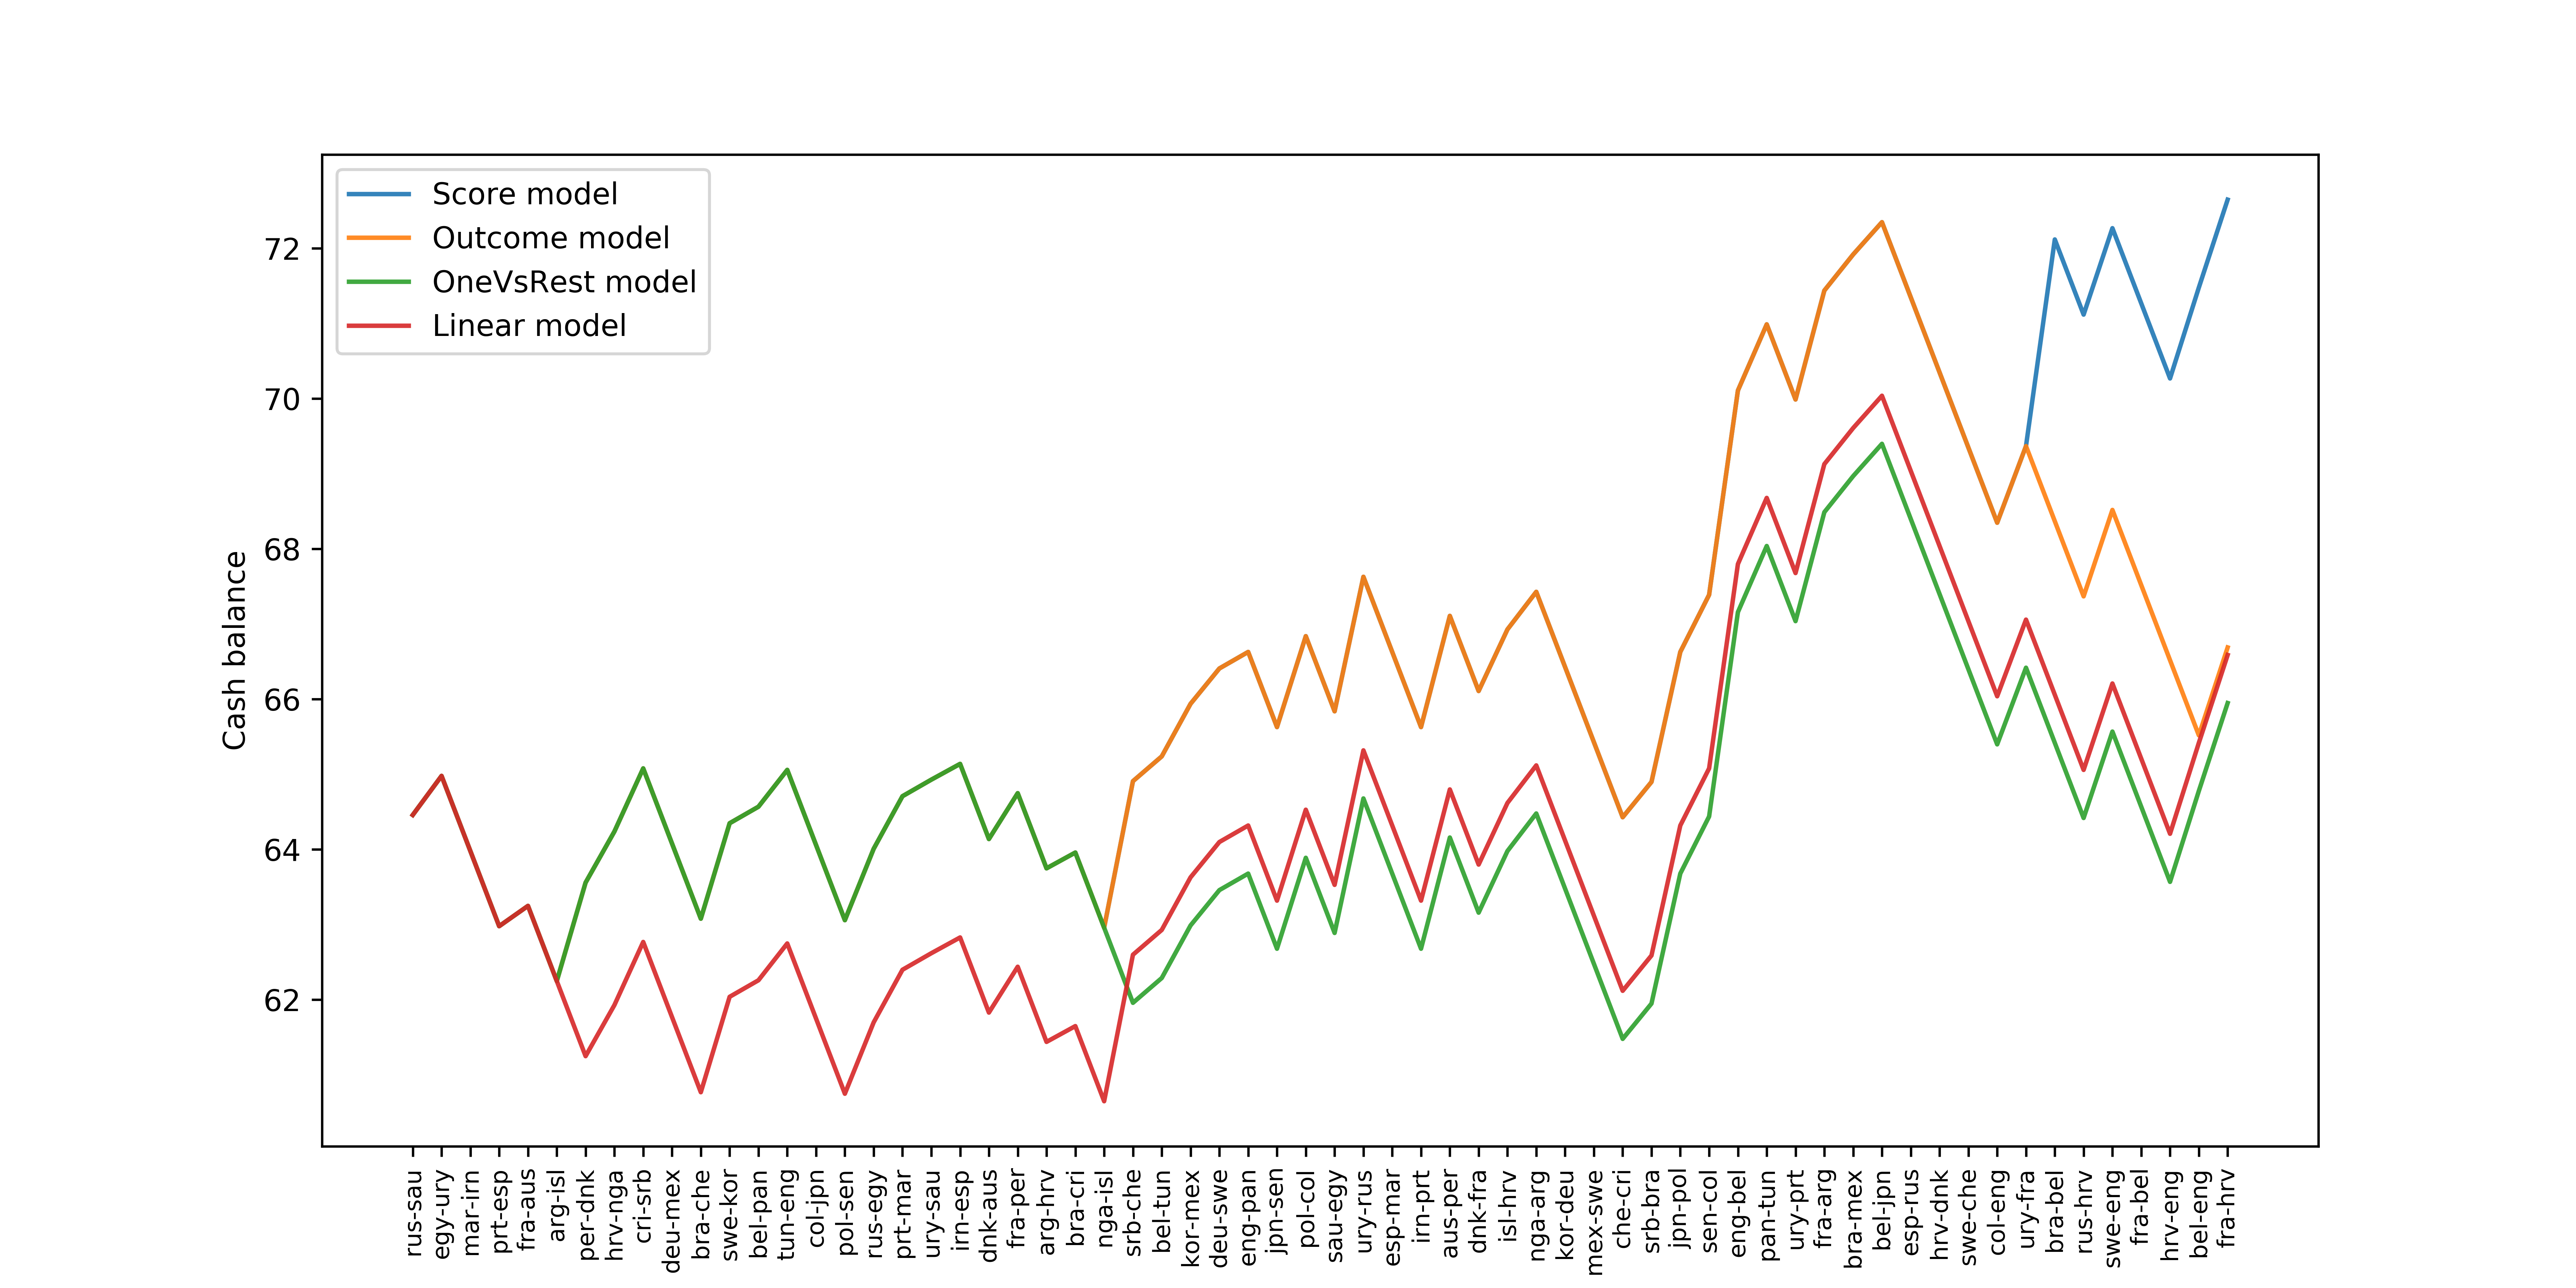
\includegraphics[width=1\textwidth]{img/match_level_2018_model_unit.png}
    \caption{Unit strategy's cash balance progression on the World Cup 2018.}
    \label{fig:unit_model_comparison}
\end{figure}

\begin{figure}[H]
    \centering
    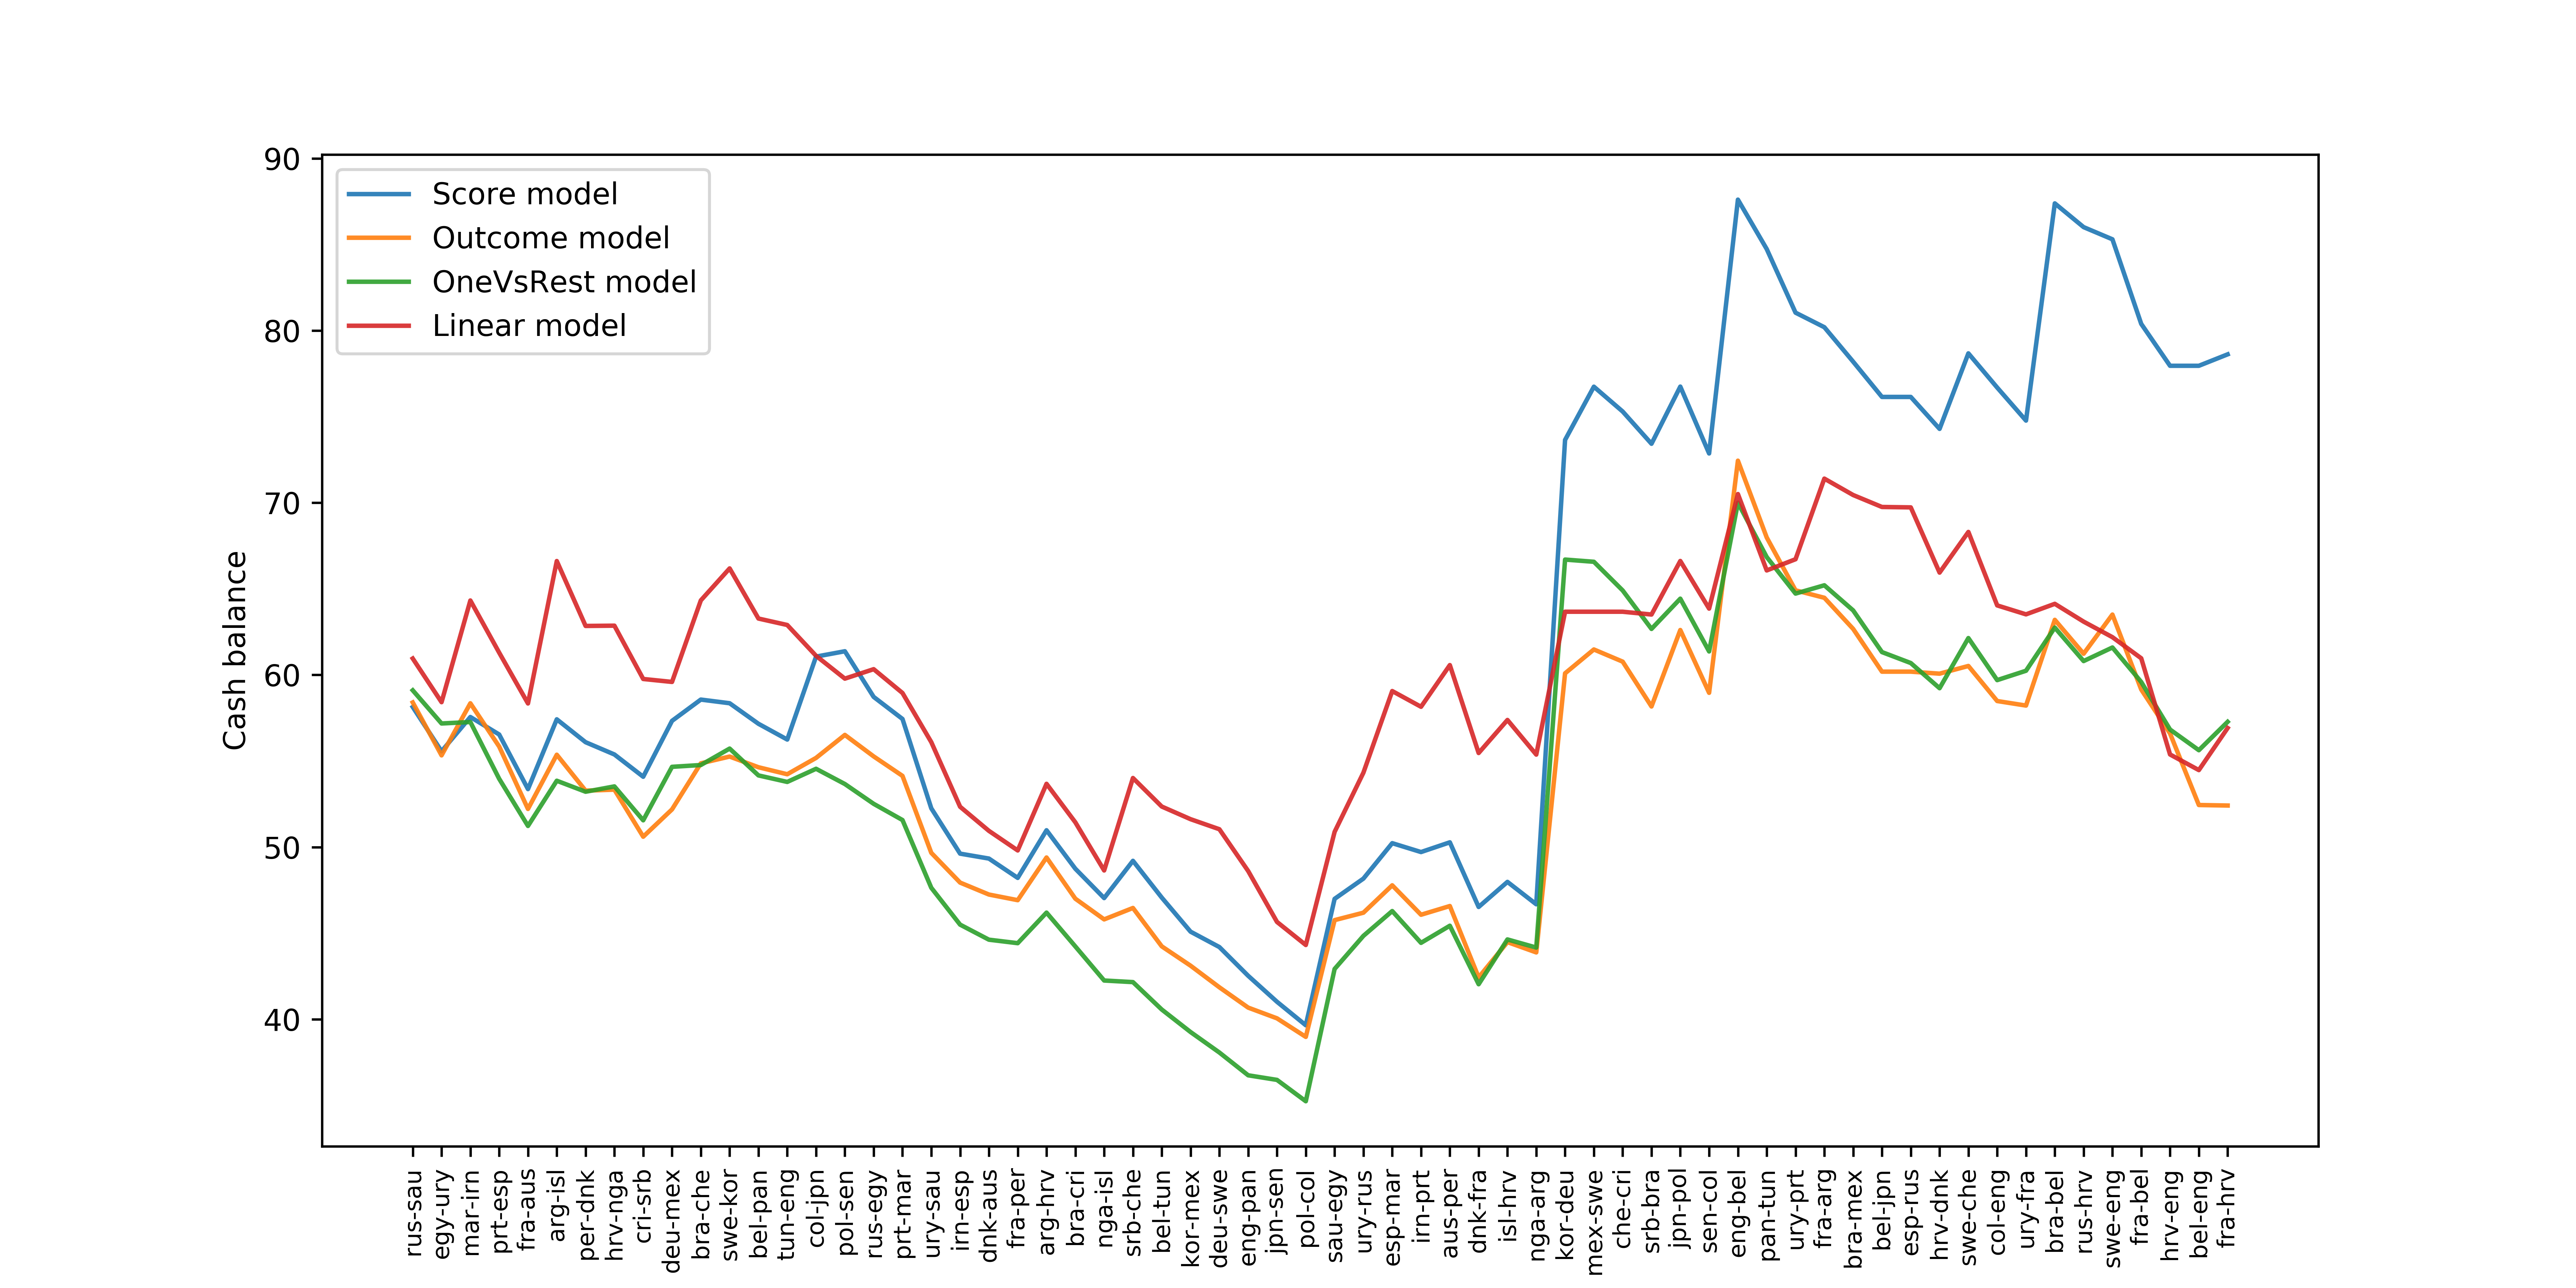
\includegraphics[width=1\textwidth]{img/match_level_2018_model_kelly.png}
    \caption{Kelly strategy's cash balance progression on the World Cup 2018.}
    \label{fig:kelly_model_comparison}
\end{figure}

\begin{figure}[H]
    \centering
    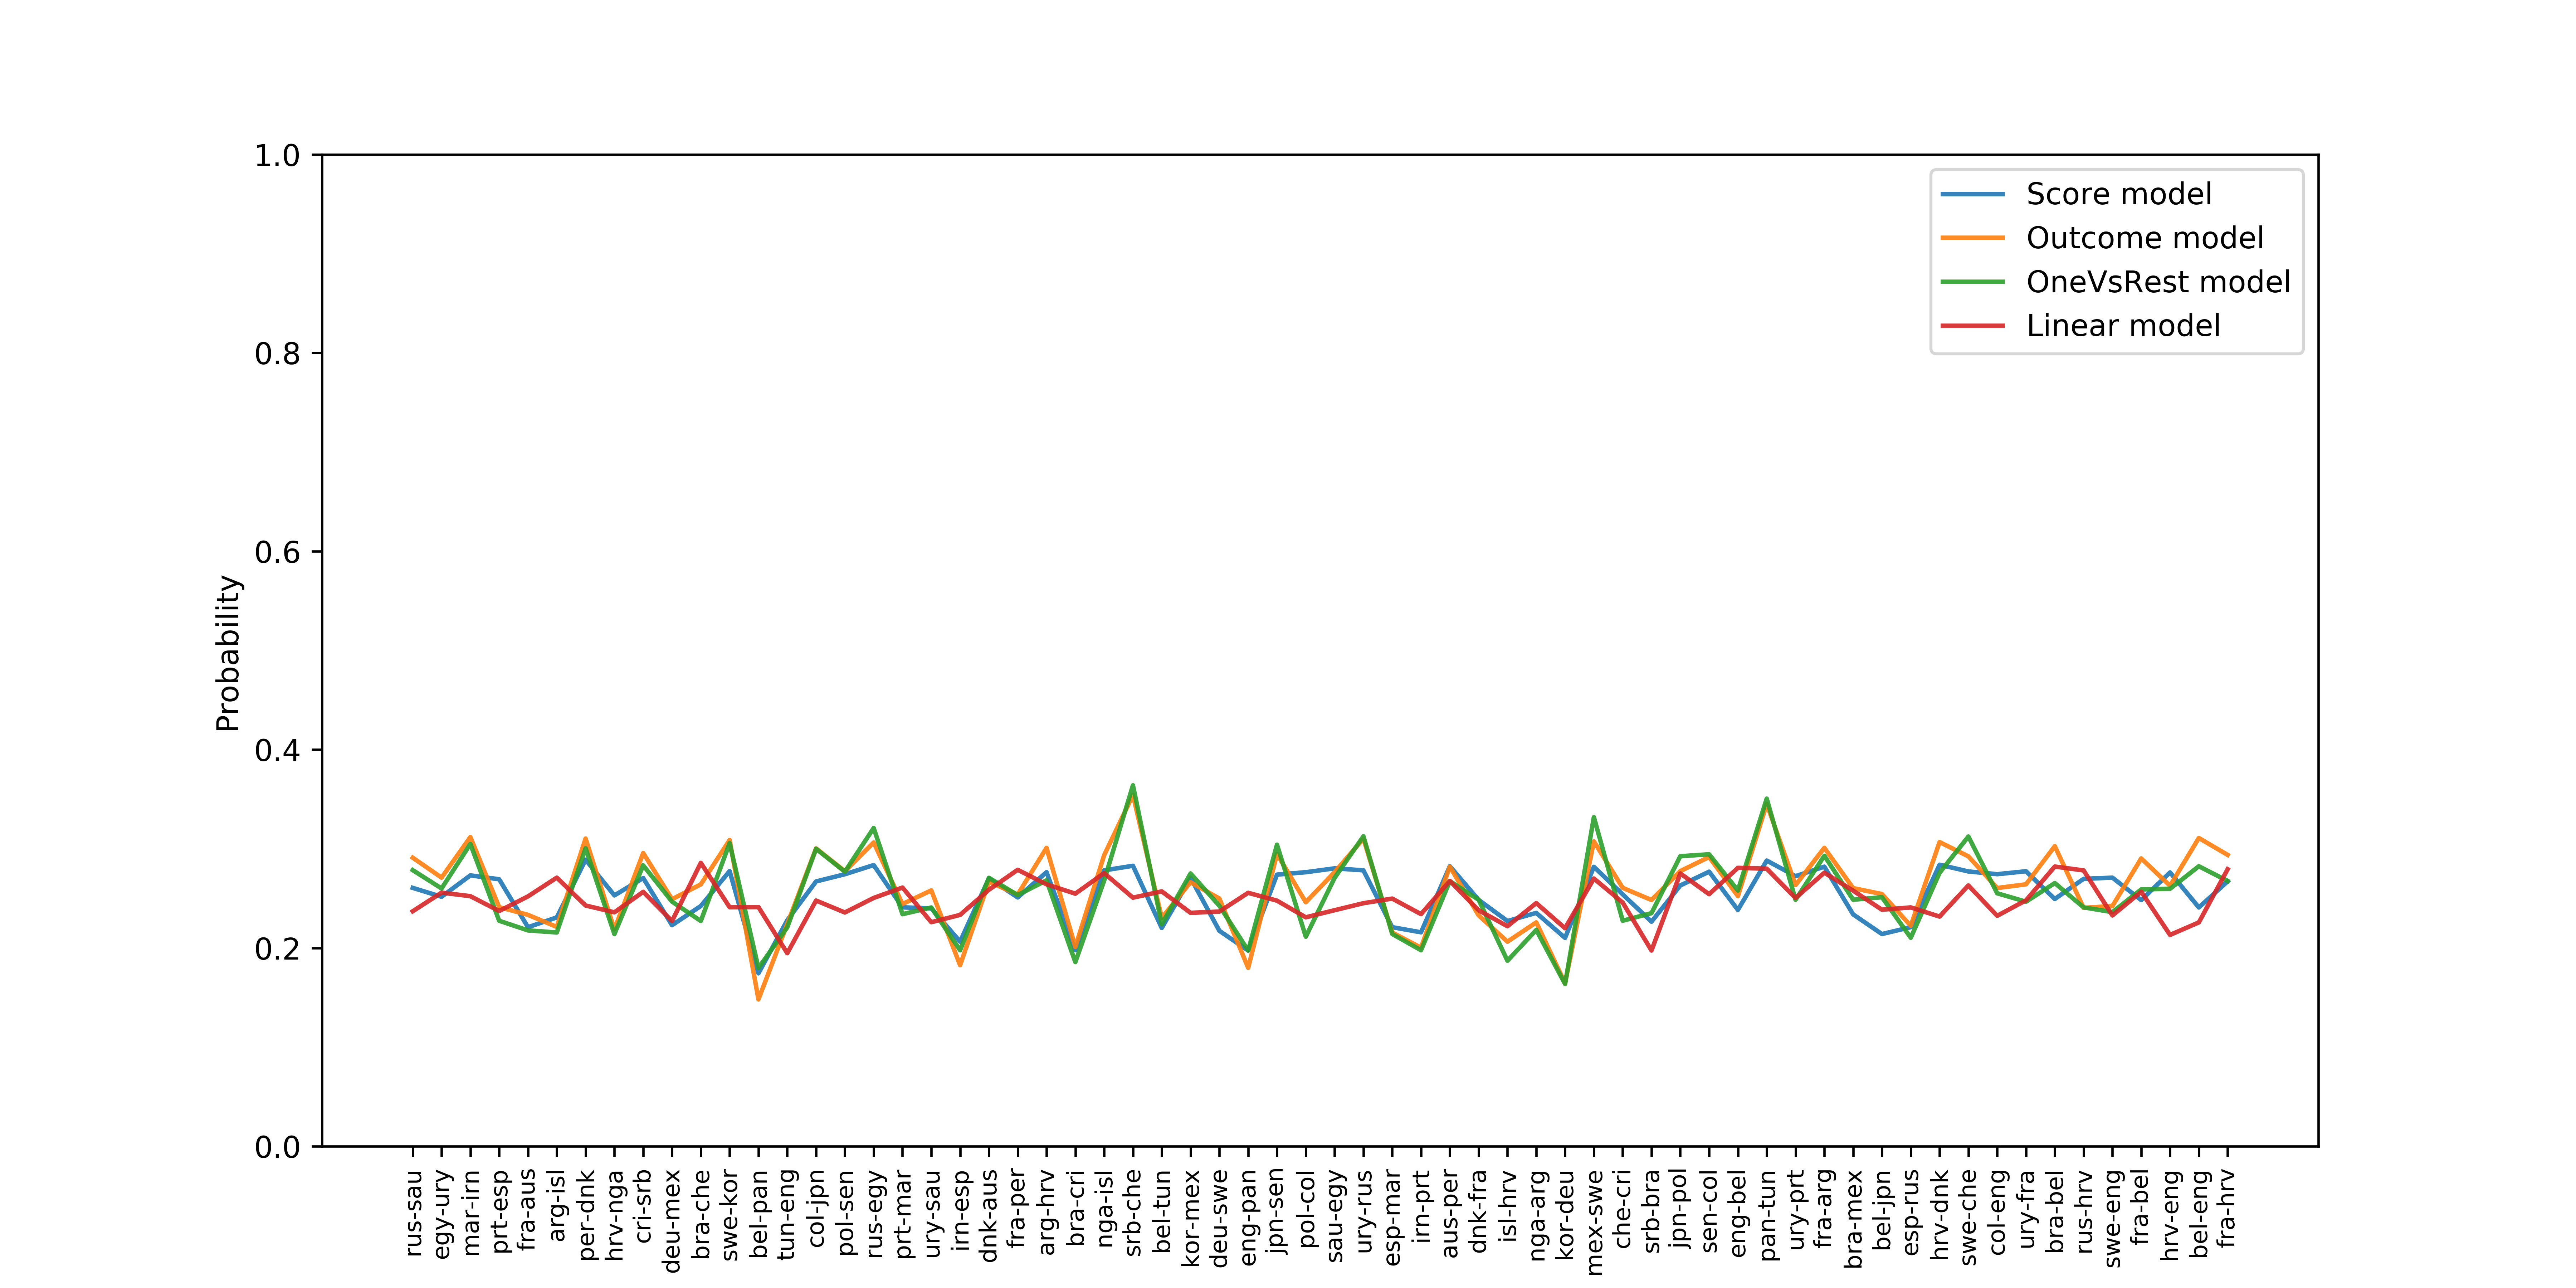
\includegraphics[width=1\textwidth]{img/match_level_2018_model_probability_draw_prob.png}
    \caption{Predicted probability of draw in the World Cup 2018.}
    \label{fig:draw_probability}
\end{figure}

\begin{figure}[H]
    \centering
    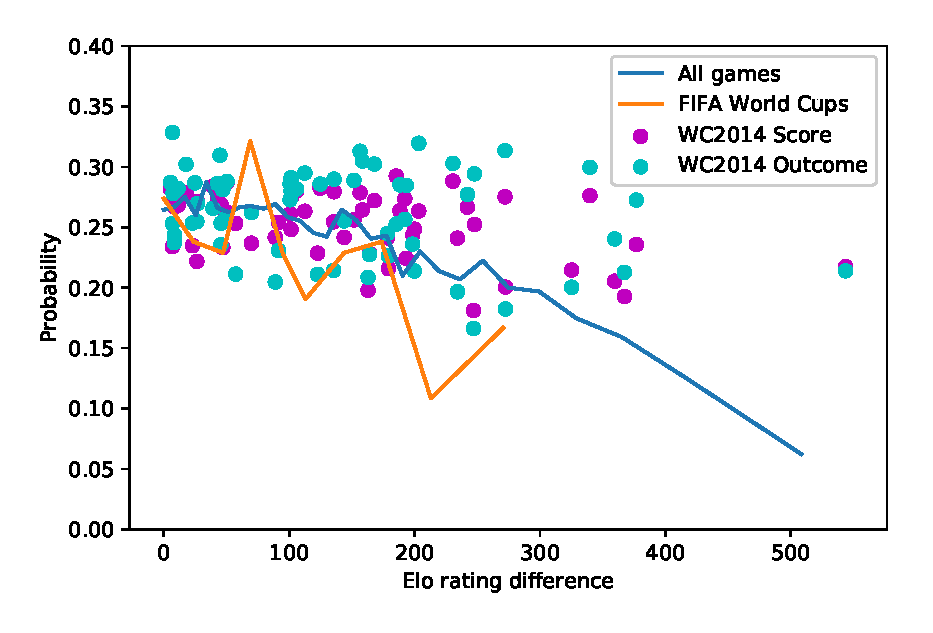
\includegraphics[width=1\textwidth]{img/draw_true_probability_wc.eps}
    \caption{The predicted probability vs. the sample probability. The sample probability of a draw is calculated from all international football games between dates 11/30/1872 - 06/04/2018. The sample probability of a draw from World Cup games is calculated based on all World Cup games between the same period. Dots are single probability estimates from \textit{Score model} and \textit{Outcome model} for matches in the World Cup 2014.}
    \label{fig:draw_prob_dist}
\end{figure}

\section{Feature set comparison}
Some of the models seem to work better with limited features. How can less describe more?

This phenomenon is visible if the models' accuracy is compared. Being one of the most important metrics, it is still not the most important for the sophisticated betting strategies like the Kelly strategy. Log loss is a metric that can be used to compare probability distributions' accuracy. A smaller value indicates a more accurate estimate. When log loss values are compared for each tournament, a model trained with a limited feature set can have a lower log loss value than the same model that is trained using all of the features. But when the average performance from every tournament is considered, training a model with all features seems to output the lowest log loss score with \textit{Outcome model} and \textit{OVR model} and second lowest (only 0.0009 difference at highest) with \textit{Score model} and \textit{Linear model}. This indicates that using all of the features benefits the probability distribution prediction, but not always the accuracy.

Random forest's feature importance value gives insight on model's reasoning. This data combined with optimal hyperparameters is one way to interpret the models since inspecting every single tree in the forest would be too cumbersome. With a random forest, an optimal value that is higher than the default for \textit{minimum samples at a leaf} can mean that some of the features are very noisy. Tree-based models, trained with generic features, seem to have a higher value for the hyperparameter \textit{minimum samples at a leaf} as we can see from Table \ref{table:hyperparam_results}. The feature importance values for \textit{Outcome model} trained with generic features are in Figure \ref{fig:outcome_feature_importance_gf}. Difference between Elo ratings is a valuable feature, but the rest of the features are harder to differentiate. Features \textit{home\_goal} and \textit{away\_goal} are the least important ones. When the importance of these features is listed for a model trained with all features (Figure \ref{fig:outcome_feature_importance_af}) \textit{home\_goal} and \textit{away\_goal} seem to rank in the middle tier.

With \textit{player features} the difference between features' importance is not as visible as it is with \textit{general features}. Features' importance is gradually decreasing feature by feature as we can see from Figure \ref{fig:outcome_feature_importance_pf}. Same features rank high with player features as they would with all features.

\begin{table}
    \caption{Optimal hyperparameters for the random forest models.}
    \resizebox{\linewidth}{!}{
    \begin{tabular}{| c  c| c| c| c|}
        \hline
        Model & Features & \# of predictors & Min samples at a leaf & Max depth\\
        \hline
        Score & AF & $\sqrt{M}$ & 1 & 8 \\
         & GF & $\log_2{M}$ & 10 & 8 \\
         & PF & $\sqrt{M}$ & 5 & Na \\
         \hline
        Outcome & AF & $\sqrt{M}$ & 3 & 8 \\
         & GF & $\log_2{M}$ & 15 & 5 \\
         & PF & $\log_2{M}$ & 3 & 8 \\
        \hline
        OVR & AF home win & $\sqrt{M}$ & 3 & 5 \\
        OVR & AF draw & $\sqrt{M}$ & 5 & Na \\
        OVR & AF away win & $\sqrt{M}$ & 3 & 5 \\
        OVR & GF home win & $\sqrt{M}$ & 10 & 12 \\
        OVR & GF draw & $\log_2{M}$ & 15 & 8 \\
        OVR & GF away win & $\log_2{M}$ & 10 & 5 \\
        OVR & PF home win & $\log_2{M}$ & 3 & 5 \\
        OVR & PF draw & $\log_2{M}$ & 15 & 5 \\
        OVR & PF away win & $\log_2{M}$ & 5 & 8 \\
        \hline
    \end{tabular}}
    \label{table:hyperparam_results}
\end{table}

\begin{figure}[H]
    \centering
    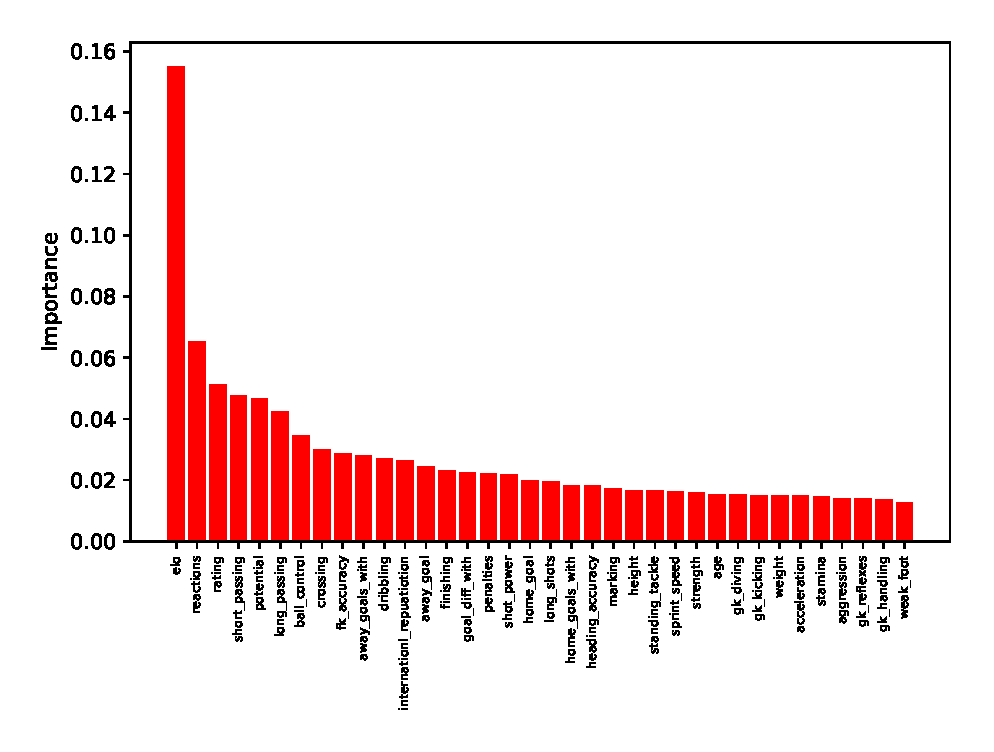
\includegraphics[width=1\textwidth]{img/match_level_2018_outcome_feature_importance_af_feature_importance.eps}
    \caption{Outcome model's feature importance with all features.}
    \label{fig:outcome_feature_importance_af}
\end{figure}

\begin{figure}[H]
    \centering
    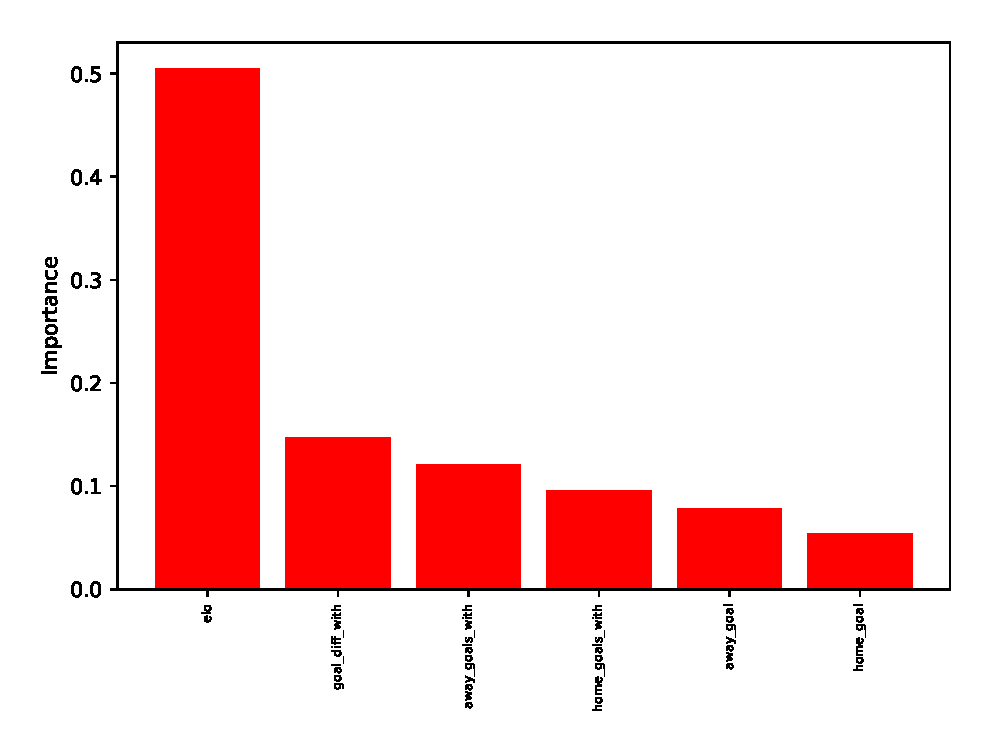
\includegraphics[width=1\textwidth]{img/match_level_2018_outcome_feature_importance_gf_feature_importance.eps}
    \caption{Outcome model's feature importance with generic features.}
    \label{fig:outcome_feature_importance_gf}
\end{figure}

\begin{figure}[H]
    \centering
    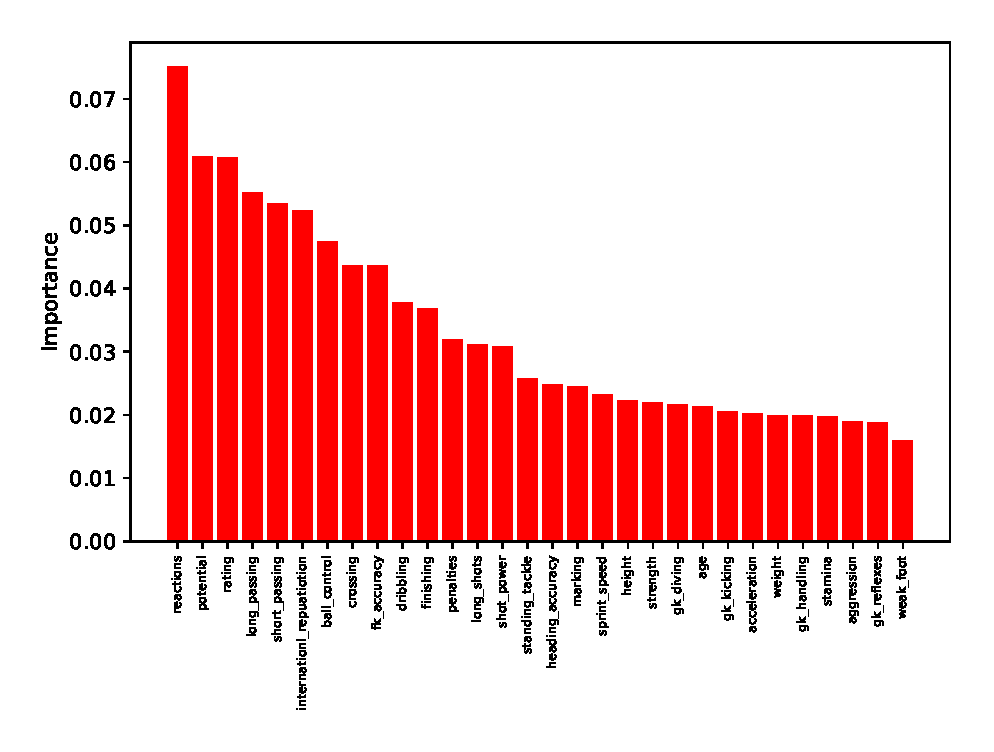
\includegraphics[width=1\textwidth]{img/match_level_2018_outcome_feature_importance_pf_feature_importance.eps}
    \caption{Outcome model's feature importance with player features.}
    \label{fig:outcome_feature_importance_pf}
\end{figure}

\section{Recursive feature elimination}
To see if using a subset of features could improve the results, recursive feature elimination (RFE) is performed for \textit{Outcome model}. The test is run two times: first time with default hyperparameters and the second time with optimal hyperparameters from the \textit{all features} setup.

The first test includes the default parameters for \textit{Outcome model}: 1000 for the number of estimators, $\sqrt{M}$ for the number of predictors, Na for the maximum depth and one for the minimum samples at a leaf node. From Figure \ref{fig:def_avg_accu} we can see that after the feature \textit{gk\_diving} is eliminated accuracy starts to decrease slowly, and from Figure \ref{fig:def_avg_loss} we can see that the log loss starts to increase. The second test's results are in Table \ref{table:outcomemodel}, and these results are visualized in Figures \ref{fig:optimal_avg_accu} and \ref{fig:optimal_avg_loss}. With this setup, the model performs better throughout the whole RFE process. Also, the model peaks the highest accuracy with only just four features. Improvement with this same feature set is not visible in the average log loss. The average log loss has a clear performance drop only when there is a single feature left.

To test the model's performance with a limited feature set we run the World cup simulation for \textit{Outcome model} using features: \textit{away\_goals\_with\_home, finishing\_diff, height\_diff, crossing\_diff, potential\_diff, fk\_accuracy\_diff, home\_goal\_mean, away\_goal\_mean, ball\_control\_diff, long\_passing\_diff,  short\_passing\_diff, reactions\_diff, rating\_diff, elo\_diff}. We chose these features since they were the smallest feature set that was able to keep the performance with the model trained with the default hyperparameters. New optimal hyperparameters are grid searched for this feature set. These hyperparameters are listed in Table \ref{table:hyperparam_results_rfe} and World Cup simulation results are in Table \ref{table:outcomemodel_rfe}. Based on the accuracy and the log loss, model's performance does not improve with the limited feature set.

Based on the progression of the average accuracy and the average log loss, models do not perform better when features are removed from the original feature set. Eventually, performance decreases but never increases during the feature elimination. Most of the time results have natural variance, which causes small changes. It seems that using every available feature does not harm random forest's performance, even though there is no guarantee that all of the features are useful. Also, RFE's suitability for this setup can be questioned, since the results are not reliable if features are correlated. Stroble et al. concluded: "In particular, the selection of the first splitting variable involves only the marginal, univariate association between that predictor variable and the response, regardless of all other predictor variables. However, this search strategy leads to a variable selection pattern where a predictor variable that is per se only weakly or not at all associated with the response, but is highly correlated with another influential predictor variable, may appear equally well suited for splitting as the truly influential predictor variable." It is possible that correlated features are ranked to be more important than the influential feature.
\begin{figure}[H]
    \centering
    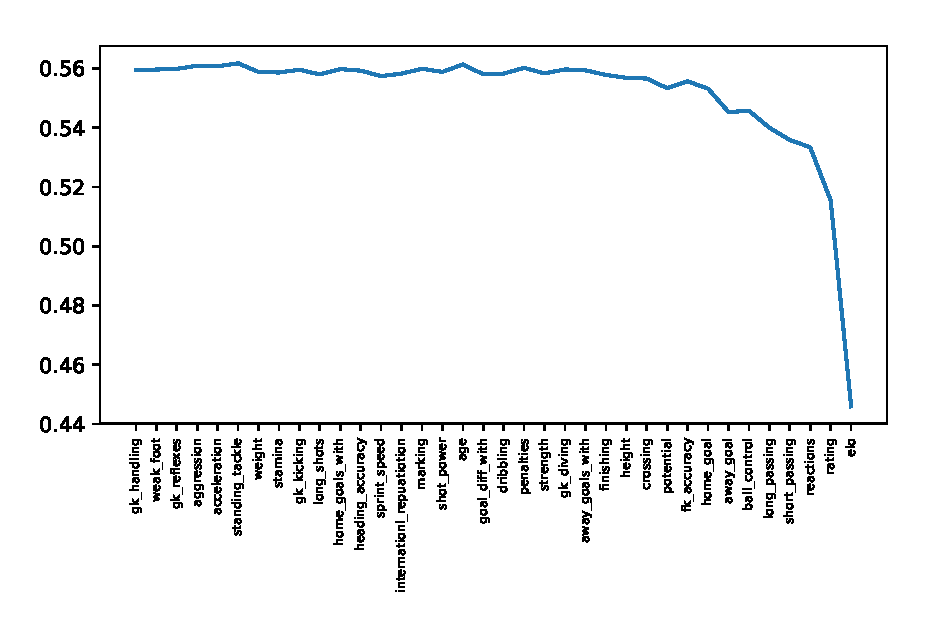
\includegraphics[width=1\textwidth]{img/default_avg_accuracy.eps}
    \caption{Mean accuracy for the recursive feature elimination on the \textit{Outcome model} with the default hyperparameters. Only the features from the first round to the 30th round are list to ensure the figure's readability.}
    \label{fig:def_avg_accu}
\end{figure}

\begin{figure}[H]
    \centering
    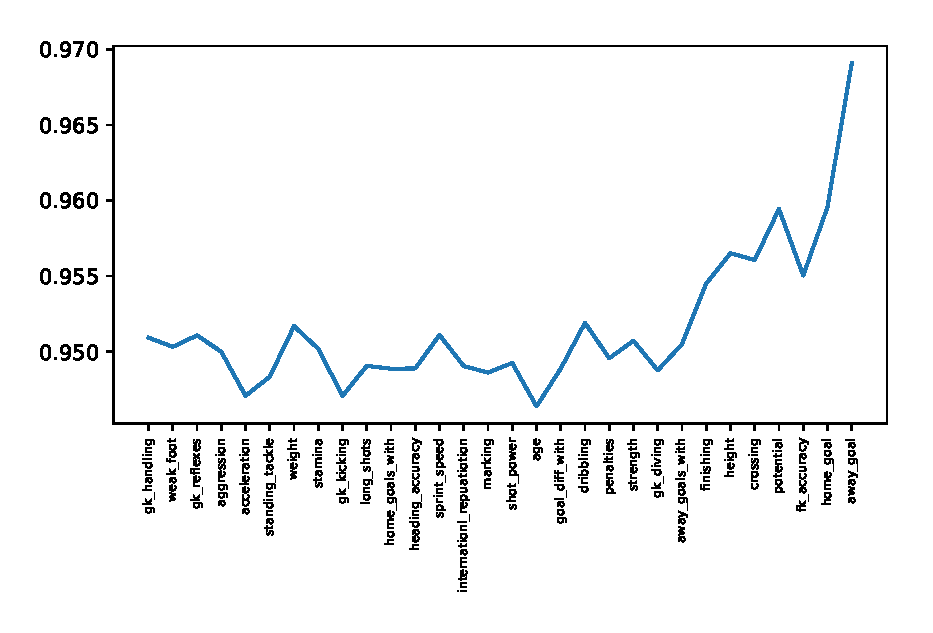
\includegraphics[width=1\textwidth]{img/default_avg_lloss.eps}
    \caption{Mean log loss for the recursive feature elimination on the \textit{Outcome model} with the default hyperparameters. Only the features from the first round to the 30th round are list to ensure the figure's readability.}
    \label{fig:def_avg_loss}
\end{figure}

\begin{figure}[H]
    \centering
    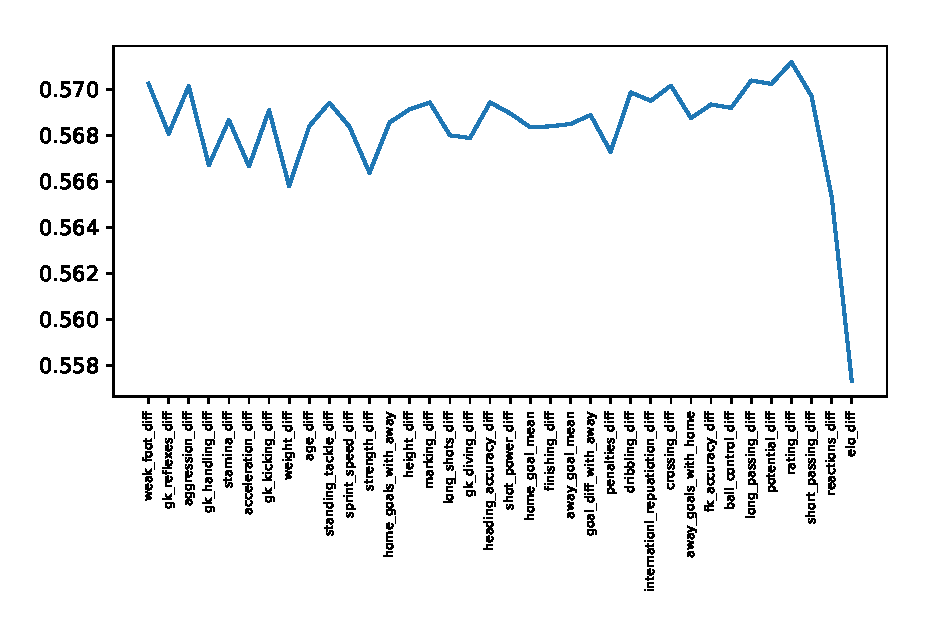
\includegraphics[width=1\textwidth]{img/optimal_avg_accuracy.eps}
    \caption{Mean accuracy for the recursive feature elimination on \textit{Outcome model}. The optimal hyperparameters from the all features setup in Table \ref{table:outcomemodel} are used.}
    \label{fig:optimal_avg_accu}
\end{figure}

\begin{figure}[H]
    \centering
    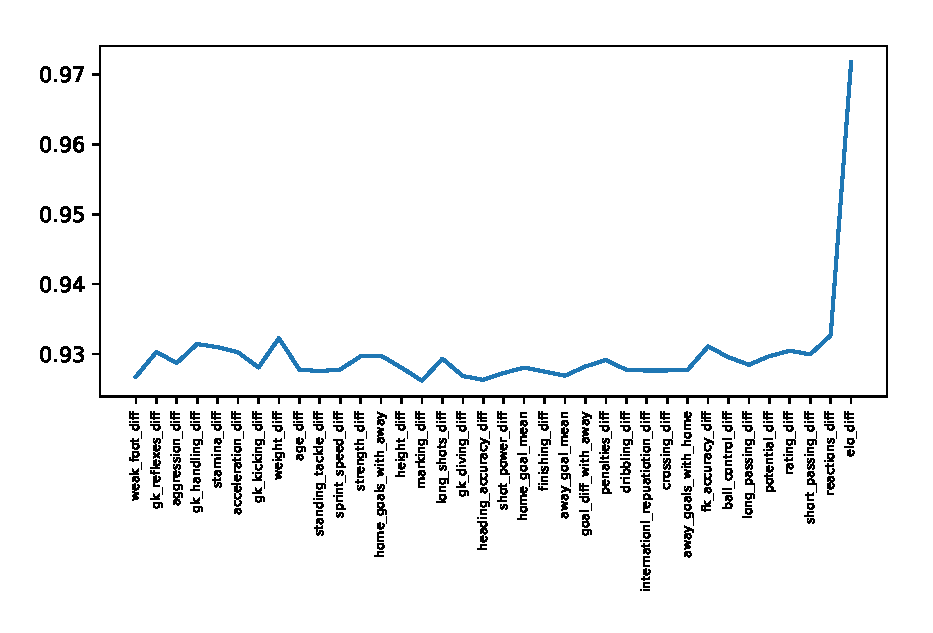
\includegraphics[width=1\textwidth]{img/optimal_avg_lloss.eps}
    \caption{Mean log loss score for the recursive feature elimination on \textit{Outcome model}. The optimal hyperparameters from the all features setup in Table \ref{table:outcomemodel} are used.}
    \label{fig:optimal_avg_loss}
\end{figure}

\begin{table}
    \caption{\textit{Outcome model's} simulation results using the limited feature set from the RFE process.}
    \resizebox{\linewidth}{!}{
    \begin{tabular}{| c | c| c| c|c|}
        \hline
        Metric& \textbf{WC 2018} & \textbf{WC 2014} & \textbf{WC 2010} & Mean\\
        \hline
        Accuracy  & 52.97\% $\pm$ 2.36 & 59.69\% $\pm$ 2.3 & 56.09\% $\pm$ 2.47& 56.25 \\
        Log Loss & 0.9953 $\pm$ 0.0087 & 0.9282 $\pm$ 0.0061 & 0.9743 $\pm$ 0.0069& 0.9659 \\
        Unit profit  & -1.79\% $\pm$ 6.16 & 14.12\% $\pm$ 6.02 & 8.82\% $\pm$ 7.47& 7.05 \\
        Kelly profit  & -37.19\% $\pm$ 11.43 & 61.45\% $\pm$ 15.42 & 77.87\% $\pm$ 12.98& 34.04 \\
 \hline
    \end{tabular}}
    \label{table:outcomemodel_rfe}
\end{table}

\begin{table}
    \caption{The optimal hyperparameters for \textit{Outcome model} trained with the limited feature set from the RFE process.}
    \begin{tabular}{| c | c| c| c|}
        \hline
         \# of predictors & Min samples at leaf & Max depth\\
        \hline
         $\sqrt{M}$ & 10 & Na \\
        \hline
    \end{tabular}
    \label{table:hyperparam_results_rfe}
\end{table}


\section{Match-level betting activity - what drives the profits?}
A model can bet on the tournament in many ways. To answer the question "What drives the profits?" it is important to see how the individual games are betted. Does the model generate a small profit in most of the games or are the profits a result from a few successful opportunities? The unit strategy gains a profit when the model predicts correctly. There is no need to analyze this in more detail, since the strategy is straightforward. Kelly strategy instead is more sophisticated and deserves a more in-depth analysis. With the requirements 1) profitable in every tournament, and 2) best average profits has \textit{Score model} trained with all features performed the best. For this reason, the following figures are plotted from \textit{Score model's} results.

The most successful tournament for \textit{Score model} was the World Cup 2018. It achieved on average 35.59\% profit. In comparison, profit from the World Cup 2014 was only 12.37\%. By the numbers performance in the World Cup 2018 was better, but what happened with match-level betting? When both of the tournaments are compared side by side in Figures \ref{fig:net_win_cost_2018} and \ref{fig:net_win_cost_2014} it is clear that a single successful bet dominates the profits in the World Cup 2018. Do not get confused by the difference in the scale of the y-axis. Total bets per match are not that different between the tournaments. Only betting frequency differs --- there are more games in the World Cup 2014 without any bets. With the World Cup 2018, the winnings are more rare but bigger. Kelly strategy gains from the abnormally high odds that are available. In the match between South Korea and Germany, the odd for South Korea's win is 19.39, even though Germany had struggled the whole tournament. With the odd as high as 19.39, the implied probability for South Korea's win is close to 5\%. These anomalous odds are certainly important, and Kelly strategy can utilize them properly. Without the three biggest winnings, this strategy would achieve small or negative profits. In the World Cup 2014, this strategy wins more often, but winnings are not as big as they are in the World Cup 2018. Steady wins would be ideal also for the World Cup 2018 but are more difficult to achieve. When winnings are more frequent predicted probabilities need to be closer to the true ones than the implied probabilities from the betting market's are. Based on the limited amount of evidence, smaller but more frequent winnings and sparser betting activity, it seems that the probability estimates for the World Cup 2014 are better than the implied ones based on the market. Whereas in World Cup 2018 profitability is based on the strategy's ability to gain from few favorable odds. A situation where abnormal odds are required for a profitable bet might be extremely hard to sustain in the long run unless betting markets provide opportunities like this often enough. Model's bias towards a higher probability of a draw compared to the market's when the difference between teams' Elo rating is relatively high is visible in both of the tournaments. This bias harms the strategy's performance.

\begin{figure}[H]
    \centering
    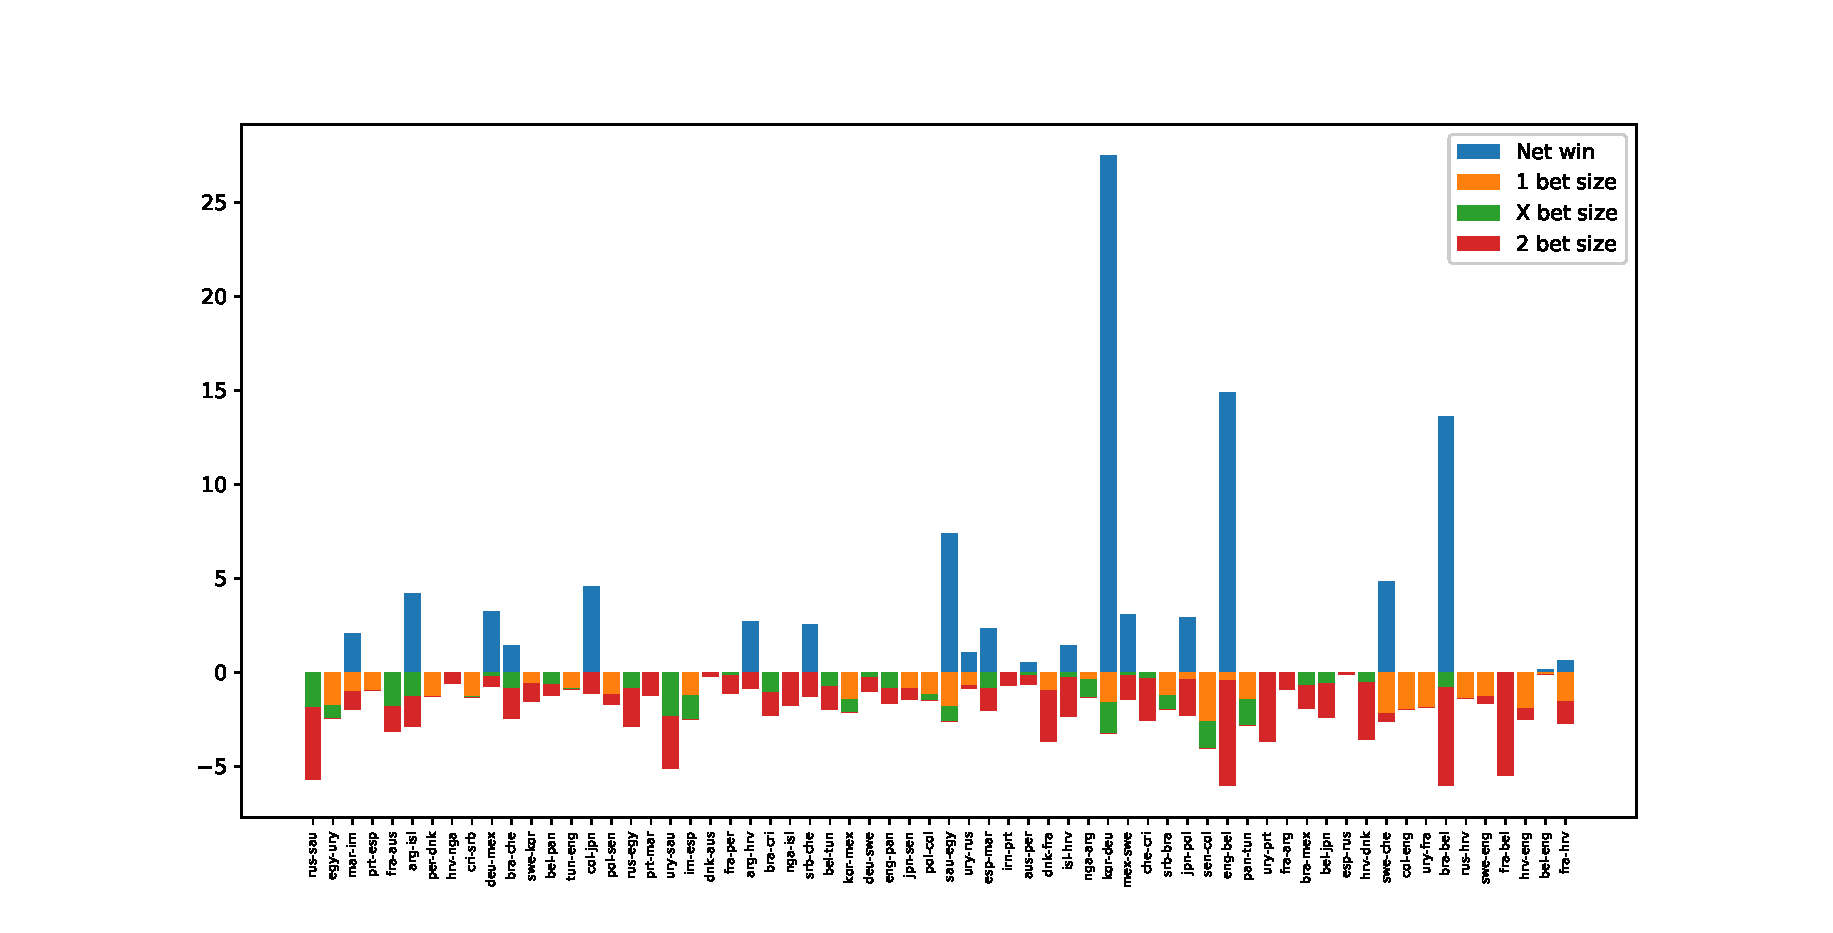
\includegraphics[width=1\textwidth]{img/match_level_2018_score_win_cost_.eps}
    \caption{Net winnings and betting costs per label for Score model in World Cup 2018.}
    \label{fig:net_win_cost_2018}
\end{figure}

\begin{figure}[H]
    \centering
    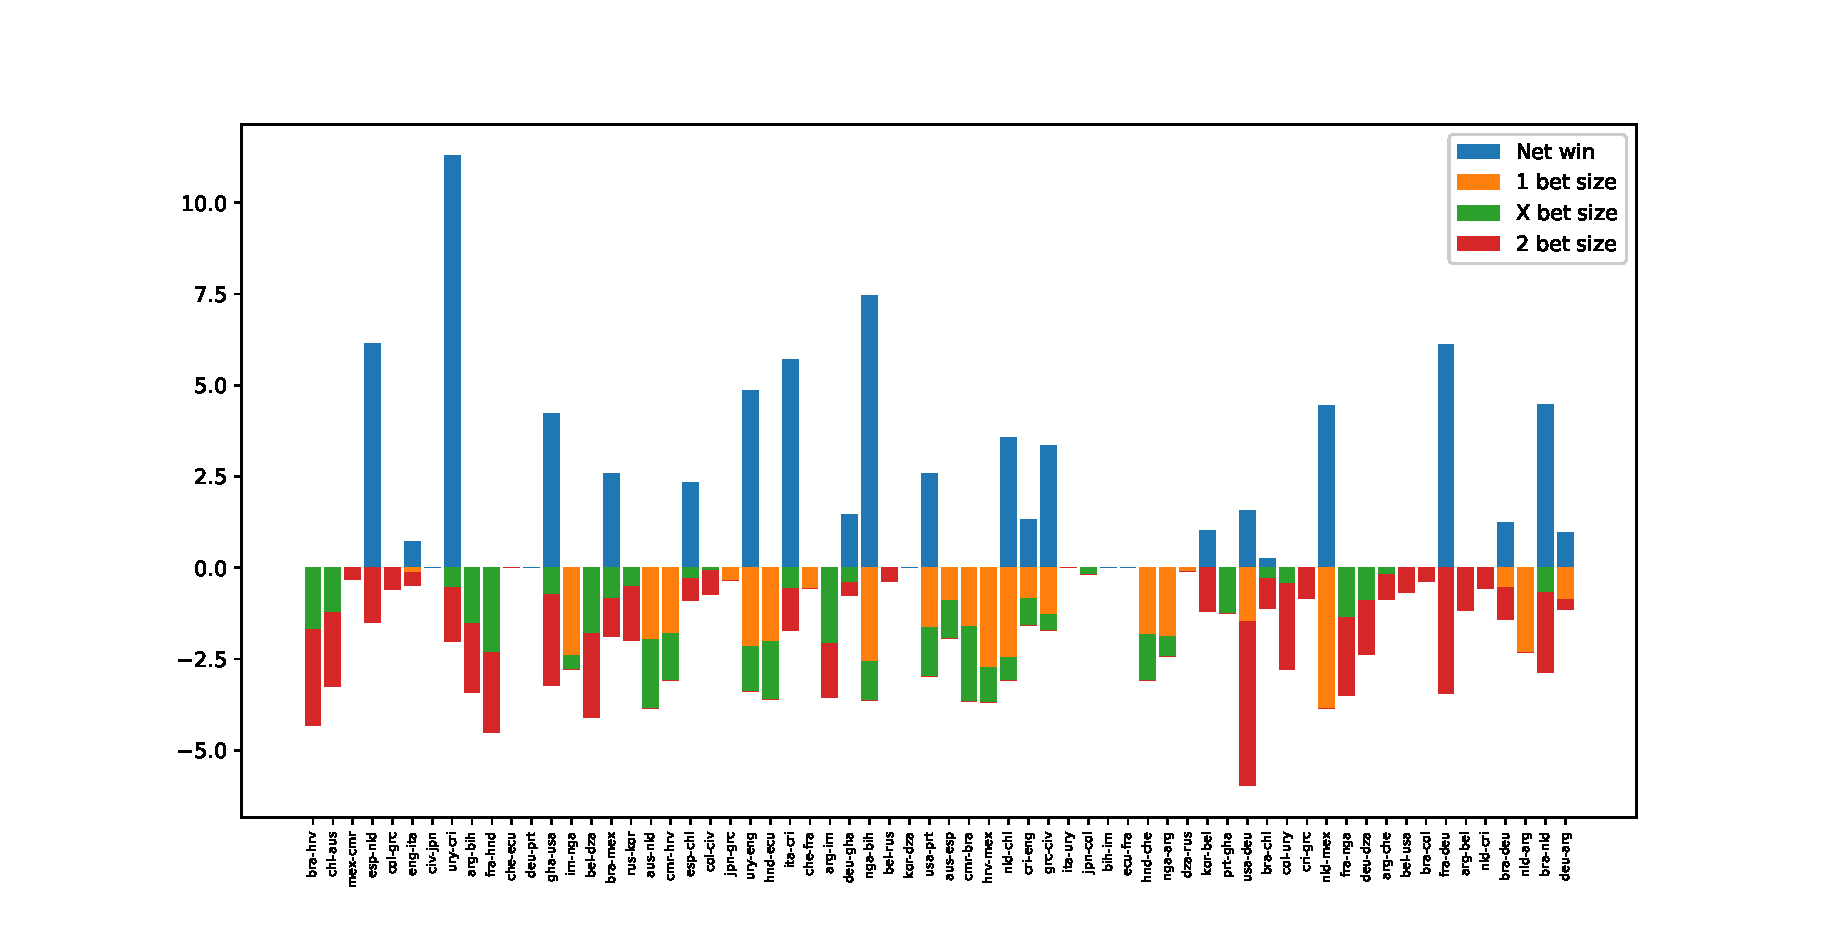
\includegraphics[width=1\textwidth]{img/match_level_2014_score_win_cost_.eps}
    \caption{Net winnings and betting costs per label for Score model trained with all features in World Cup 2014.}
    \label{fig:net_win_cost_2014}
\end{figure}

\section{Summary}
In total there are 12 model and feature set combinations. In every tested World Cup tournament over half of the models perform better than the bookmaker's model. \textit{Score model} trained with all features is the best model in performance. Its average return in all of the tournaments is 24.05\%. From the models \textit{Outcome model} trained with player features can generate profit from all of the tournaments using both of the betting strategies.

All of the models predict the probability for a home win and an away win very similarly. Probability estimates for a draw differ the most between the models. \textit{Outcome model} and \textit{OVR model} are more aggressive with the predictions while \textit{Score model} and \textit{Linear model} predict values closer to the average. All of the models miss most of the draws and very seldom give the highest probability for that class. Based on the implied probabilities bookmakers behave similarly.

Using a subset of the whole feature set improved the accuracy and the profits only for a single tournament. No subset was able to improve the results in all of the tournaments. Results from recursive feature elimination imply that the accuracy and the log loss score did not improve during the feature elimination process. With the whole feature set models can achieve the lowest log loss value or the second lowest log loss value with only a minimal difference to the best one. This constantly low log loss value indicates that using all of the available features is the best way to train any of the models.

The individual winnings differ between the World Cup 2018 and the World Cup 2014; winnings are more significant but rarer during the World Cup 2018. If this is the trend, meaning that during the upcoming tournaments finding a suitable odds to bet on is even harder, winnings become even more rare or non-existing.
